% !TEX encoding = UTF-8 Unicode

\documentclass[10pt]{amsbook}
\usepackage[b5paper]{geometry}
\usepackage{kerbal-book}
\usepackage{graphicx}

\usepackage{tikz}
\usepackage{pgfplots}

%\usepackage[korean]{babel}


%\setlength{\voffset}{- 0.3 in}
\setlength{\footskip}{40pt}

\setlength{\parindent}{1.2em}
\setlength{\parskip}{0.8em}
\renewcommand{\baselinestretch}{1.5}

\newcommand{\dia}{$\diamondsuit$}


\title{kerbal-book}
\author{Alberto Liberio Humaniense Disciplino}
\date{March 2016}

\begin{document}

\maketitle
\sf
%\frontmatter
\chapter*{Kerbal Space Program이란?}
\tableofcontents
%\mainmatter
\part{시작하기}
\chapter{궤도에 올리기}
\section{운동에너지 얻기}
\section{공기저항}
\section{공기역학 및 안정성}
\subsection{Over-compensating}
\section{재진입시 주의사항}
\subsection{방열판 (Heat Shield)}
\subsection{낙하산 (Parashute)}

\begin{tabular}{|c|c|c|}
이름&작동속도&면적
\end{tabular}
\chapter{다단 로켓과 $\Delta v$}
\section{연료}

\begin{align}
    \Delta v =I_{sp}\, g_0\log\frac{M+m}{M}
\end{align}

\begin{align}
    \Delta v = I_{sp}\, g_0\log\frac{M+(1+\alpha) m}{M+\alpha m}
\end{align}
\begin{align}
    \Delta v \rightarrow I_{sp}\, g_0\log(1+\alpha^{-1})
\end{align}

is independent of thrust force but only depend on isp and etc

Let's assume $I_{sp} =320 s$ and 

Estimated Engine Mass / Fuel Mass = 1/6

Estimated Fuel Tank Mass / Fuel Mass = 1/8

$\Delta v = 4669.78 m/s$

실제로는 1단의 경우 공기저항으로 인해 연료를 많이 실을 수록 오히려 얻을 수 있는 운동에너지가 줄어드는 결과를 보이기도 한다. 따라서 많은 양의 화물(Load)을 쏘아 올리기 위해서는 `다단 로켓 (multi-stage rocket)'과 `아스파라거스 로켓 (asparagus-staging rocket)'이 필요하다.


%{\fontfamily{omyglm}가나다}
%{\fontfamily{omyglm}\selectfont가나다}
%{\fontfamily{unbtbco04}\selectfont가나다}
\section{다단 로켓 (Linear Staging)}
a


\section{아스파라거스 (Asparagus Staging)}

\section{$I_{sp}$}
\begin{align}
I_{sp} = \frac{F}{\dot{m}g_0}
\end{align}


\chapter{궤도운동}
\section{용어설명 및 주의사항}
*근일점은 꼭 태양과 지구사이만의 의미가 아니고 일반적으로 사용할것임
\section{원궤도}
\section{타원궤도}
별 (start) 우주선 (projectile) 위치에너지 (potential energy)
\begin{align}
&r^2 \dot{\theta} = l
\\&\ddot{r}-\frac{l^2}{r^3}+\frac{GM}{r^2} = 0
\end{align}
\begin{align}
	-l^2r^{-2}\frac{d^2r^{-1}}{d\theta^2}-l^2r^{-3}+GMr^{-2} = 0
\end{align}
\begin{align}
	\frac{d^2r^{-1}}{d\theta^2}+r^{-1}-GMl^{-2} = 0
\end{align}

이러한 우주선(projectile)의 운동방정식의 해는 다음과 같다.
\begin{align}
	r^{-1} = \frac{GM}{l^2} + \sqrt{\frac{2\epsilon}{l^2}+\left(\frac{GM}{l^2}\right)^2}\cos(\theta+\theta_0)
\end{align}
여기서 $\epsilon$은 우주선(projectile)의 질량당 총 에너지이다. 이러한 식은 이차곡선(원, 타원, 포물선, 쌍곡선)을 나타내는 표현이다. 따라서 이는 역제곱힘에서의 궤도가 이차곡선이 된다는 증명이다.
이 식을 $l$과 $\epsilon$이 아닌 $l$과 근일점($r_p$)의 함수로 나타내면 다음과 같이 나타낼 수도 있다.
\begin{align}
	r^{-1} = \frac{r_p^{-1}}{2}\cdot\frac{1}{1+\epsilon (GM)^{-1}r_p} +\frac{r_p^{-1}}{2}\cdot\frac{1+2\epsilon (GM)^{-1}r_p}{1+\epsilon (GM)^{-1}r_p}\cos(\theta+\theta_0)
\end{align}
$r$이 무한대로 가지 않고 유한한 영역에서 진동하고 있으면 원이나 타원, 즉 구속궤도(bound orbit)이 되고, $r$이 무한대, 즉 $r^{-1}=0$인 지점이 있으면 비구속궤도(unbounded orbit)가 될 것이다.

\section{쌍곡선궤도 - 탄성충돌}
\section{슬링샷}

\begin{align}
	\Delta \theta = \pi + 2\sin^{-1}\frac{1}{{1+2\epsilon (GM)^{-1}r_p}}
\end{align}

\paragraph{특정 기준계에 대한 슬링샷 결과}
어떤 기준계에 대해서 우주선의 입사 속도가 $\vec{v}_s(t=-\infty)$, 천체의 속도가 상수 $\vec{v}_c$라고 한다면, 위와 같은 계산결과에 따라 우주선의 최종 속도가 어떻게 되는지 계산해보자.

우선 천체계에서 우주선의 속도는 $\vec{v}_s(t=-\infty)-\vec{v}_c$가 될 것이다.

예) 달을 이용한 가속
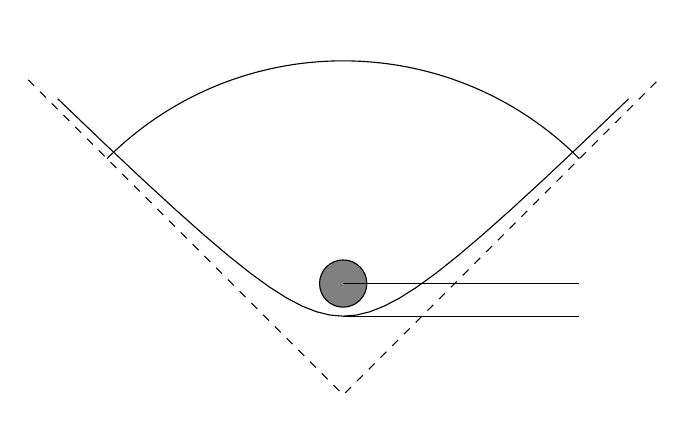
\begin{tikzpicture}
\draw[fill=gray] (0,{sqrt(2)}) circle (.3);
\draw [dashed] (-4,4)--(0,0)--(4,4);
\draw plot[domain=-2:2, thick] ({sinh(\x)},{cosh(\x)});
\draw (0,{sqrt(2)})--(3,{sqrt(2)});
\draw (0,1)--(3,1);
\draw[thin] (-3,3) arc (135:45:{3*sqrt(2)});
\end{tikzpicture}

진입속도 $v$, 근접거리 $r$.

\chapter{달 미션}

\part{매뉴버}
\part{미세조정 (Fine-tuning)}
\part{행성간 비행}
\chapter{시간계획 정하기}
\chapter{포획 (Capturing)}
행성계 외부에서 진입하는 물체는 탈출속도를 넘어서므로\footnote{정확히는 `행성계 관점에서 보았을 때 양(陽)의 에너지를 갖으므로'라고 하는 것이 옳을 것이다. `탈출속도'라는 개념은 보통 원궤도를 그리던 물체에 얼마만큼의 $\Delta v$가 주어져야 탈출할 수 있는지에 대한 얘기이다.} 힘이 작용하지 않으면 쌍곡선 궤도를 그리며 다시 행성계 밖으로 탈출하게 될 것이다.
안정적인 미션 수행을 위해서 행성간 미션에서는 도착지에서 충분히 감속하여 구속궤도를 만들 수 있는 기술이 필요하다. 이를 `포획'이라고 부르도록 하겠다. 포획이 이루어지지 않는다면 행성의 인공위성 궤도에 진입하는 미션을 수행할 수 없으며, 착륙 미션에 경우 한번만에 성공해야 하는 부담을 안게 된다.\footnote{비구속궤도(쌍곡선궤도)로부터 대기권으로 진입할 때, 높은 진입속력으로 인해 높은 열이 발생하게 되어 우주선이 소실될 위험성이 커지게 되며, 또한 다시 튕겨나가지 않고 충분히 감속할 수 있는 가능성도 줄어들게 된다.}

엔진을 이용한 능동적인 감속은 설명이 필요없으므로 여기서는 동력을 사용하지 않고 포획당하는 방법에 대해서 설명하고자 한다. 두가지 방법을 생각할 수 있을텐데, 행성의 대기를 이용한 방법과 행성의 위성을 이용한 방법이 있을 것이다. 각각의 방법에 대해서 설명하고자 한다.
\section{대기를 이용한 포획 (Atmospheric Capture)}
\section{위성을 이용한 포획 (Sling-shot Capture)}
다음은 위성을 이용한 슬링샷으로 행성계에서의 속도를 줄일 수 있는지 검토해 보도록 하자. 위성과 조우시 위성의 속도가 우주선의 반대방향이라면 위성의 운동량을 받아 감속할 수 있으리라고 예상할 수 있을 것이다. 하지만 행성간 여행에서 그렇게 정확한 타이밍을 맞출 수 있으리라고 기대하기는 어렵다. 이번 section에서는 행성계 진입후 주어진 상황에서 감속할 수 있는지에 대해 알아볼 것이다. 다음 section에서는 진입 타이밍을 조정하는 법에 대해 논의해 보겠다.

우선 행성과 위성은 충분히 멀리 떨어져 있어서 조우(encounter)를 탄성충돌로 근사할 수 있다고 가정할 것이다. 사실 KSP는 각 천체의 '영향권'내에서 1체문제로 환원함으로서 이러한 가정을 충실히 따르고 있다.
\section{포획을 위한 궤도조정 (Fine-tuning with Sling-shot Capture)}

\chapter{사례들}
\section{Juno's Maneuver}
\begin{enumerate}
\item 지구계를 탈출한다.
\item 약 2배의 공전궤도를 만들어 다시 지구와 만날 수 있게 한다.
\item 원일점에서 근일점을 낮게 하는 매뉴버를 실시하여 다음 매뉴버에서의 에너지 효율을 높인다.
\item 지구를 이용한 슬링샷 효과를 포함하여 목성과의 접점을 만든다.
\item 목성근체에서 목성과 비슷한 속도로 가속하여 목성궤도로 들어간다.
\end{enumerate}
\part{다루어지지 않은 것들}

\chapter{3체 문제 (Three Body Problem)}
\section{KSP의 간략화}
\section{근일점 변화}
\begin{align}
	\frac{d^2r^{-1}}{d\theta^2}+r^{-1}-GMl^{-2}-l^{-2}r^2V'(r) = 0
\end{align}
\begin{align}
	\frac{d^2r^{-1}}{d\theta^2}+r^{-1}-GMl^{-2}+2 l^{-2}r^3 \left(\frac{|\alpha_-| -|\alpha_+|}{2}+\frac{|\alpha_-| +|\alpha_+|}{2}\cos(\theta-\omega t)\right)= 0
\end{align}
\section{세차운동}
*로켓발사로 인한 변화
\\*애초에 축은 0도로 고정
\chapter{상대론적 문제}
\section{특수상대론: 로렌츠변환}
\section{특수상대론: 적색/청색편이}
\section{일반상대론적 효과 및 천체모델의 근사성}
\part{천체 데이터 및 프로토콜}
\backmatter
\backpage

\end{document}
